\section{Relativistic combustion}
This chapter of the lecture notes is largely based on the references
% According to Hindmarsh, abbreviating "references" as "refs" is OK in the thesis.
\cites{hindmarsh_gw_pt_2019}{espinosa_energy_2010}.
\todo{Add more content from \cite[ch. 6]{mazumdar_review_2019}.}

If the wall velocity is constant, \eqref{eq:ep_conservation_total} also holds in the wall frame.
Therefore for a wall moving in the z-direction
\cite[eq. 7]{espinosa_energy_2010}
\begin{equation}
\partial_z T^{zz} = \partial_z T^{z0} = 0.
\end{equation}
Inserting the definition of $T$ from \eqref{eq:ep_tensor} results in the
bubble wall junction conditions
\cites[eq. 7.22]{lecture_notes}[eq. 135.2, 135.3]{landau_fluid_1987}
% This is almost trivial.
\begin{align}
w_- \tilde{\gamma}_-^2 \tilde{v}_- &= w_+ \tilde{\gamma}_+^2 \tilde{v}_+,
\label{eq:junction_condition_1} \\
w_- \tilde{\gamma}_-^2 \tilde{v}_-^2 + p_- &= w_+ \tilde{\gamma}_+^2 \tilde{v}_+^2 + p_+
\label{eq:junction_condition_2}
\end{align}
The first junction condition can be trivially rearranged to
\begin{equation}
w_- = \frac{\tilde{\gamma}_+^2 \tilde{v}_+}{\tilde{\gamma}_-^2 \tilde{v}_-} w_+,
\label{eq:wm_junction}
\end{equation}
which we will need later.

The junction conditions can be rearranged as
\cites[eq. 7.32]{lecture_notes}[eq. 4.134]{rezzolla_relativistic_2013}
\todo{According to Giese these are from Landau \& Lifschitz, Fluid Mechanics}
\todo{How to prove this step? My attempts of manual proof have failed.}
\begin{align}
\tilde{v}_+ \tilde{v}_- = \frac{p_+ - p_-}{e_+ - e_-} \\
\frac{\tilde{v}_+}{\tilde{v}_-} = \frac{e_- + p_+}{e_+ + p_-}
\label{eq:junction_ep}
\end{align}
Further simplification of these requires additional definitions
that we will now introduce.

% -----
% Transition strength
% -----

The trace of the energy-momentum tensor of \eqref{eq:ep_tensor} is
% The tr() notation is not correct, as it does not account for the metric.
\begin{align}
% \text{tr} (T^{\mu \nu})
% &=
T^\mu_\mu
&= g_{\mu \nu} T^{\mu \nu} \\
&=3p - e
\end{align}
We can quantify its difference from zero with the trace anomaly
\cites[eq. 7.24]{lecture_notes}[eq. 28]{giese_2020}
\begin{equation}
\theta \equiv \frac{1}{4}(e-3p).
\label{eq:theta}
\end{equation}
The definition of the trace anomaly varies by a factor of $\frac{1}{4}$ depending on the source as a matter of convention.
To alleviate this confusion, we introduce the trace anomaly without the factor of $\frac{1}{4}$ as
\begin{equation}
\Theta \equiv e - 3p.
\label{eq:theta_big}
\end{equation}
The difference of a quantity $X$ just ahead and behind the wall is denoted as
\begin{equation}
\Delta X
\equiv X_+(T_+) - X_-(T_-) % \\
% &= \theta_s(w_s) - \theta_b(w_b).
\end{equation}
The difference of a quantity $X$ in both phases at the same temperature is denoted as
\begin{equation}
DX_\pm \equiv X_+(T_\pm) - X_-(T_\pm),
\end{equation}
where $\pm$ means that we can compute this quantity at either $T_+$ or $T_-$.
The difference of a quantity $X$ in the same phase at different temperatures is denoted as
\begin{equation}
\delta X_\pm \equiv X_\pm(T_+) - X_\pm(T_-).
\end{equation}
These are related by
\begin{align}
\Delta X
&= X_+(T_+) - X_-(T_-) \\
&= \left( X_+(T_+) - X_-(T_+) \right) + \left( X_-(T_+) - X_-(T_-) \right) \\
&= DX_+ + \delta X_-.
\label{eq:delta_relation}
\end{align}
With these we can define the transition strength
\begin{equation}
\alpha_+
\equiv \frac{4 \Delta \theta}{3 w_+}
= \frac{4}{3} \frac{\theta_+(T_+) - \theta_-(T_-)}{w_+}
\label{eq:alpha_plus}
\end{equation}
and the transition strength at nucleation temperature
\cite[eq. 2.11]{hindmarsh_gw_pt_2019}
\begin{equation}
\alpha_n
\equiv \frac{4D\theta(T_n)}{3w_n}
= \frac{4}{3} \frac{\theta_+(T_n) - \theta_-(T_n)}{w_n}.
\label{eq:alpha_n}
\end{equation}
A quantity similar to the trace anomaly is the pseudotrace
\cites[eq. 34]{giese_2020}[eq. 1]{giese_2021}
\begin{equation}
\bar{\Theta} \equiv e - \frac{p}{c_{s,b}^2}.
\label{eq:theta_bar}
\end{equation}
It is defined with respect to $c_{s,b}^2$ in both phases so that eq. \ref{eq:junction_conditions_simplified} can be simplified.
It should be noted that the articles \cites{giese_2020}{giese_2021} denote this pseudotrace as $\bar{\theta}$,
but we have chosen the symbol $\bar{\Theta}$ in accordance with \eqref{eq:theta_big} to highlight that it doesn't have the factor of $\frac{1}{4}$ as \eqref{eq:theta} does.
Using it we can define the transition strength for the pseudotrace,
sometimes denoted as $\alpha_{\bar{\Theta}}$, as
\todo{Is this the optimal phase transition strength for detonations?}
\cites[eq. 34]{giese_2020}[eq. 1]{giese_2021}
\begin{equation}
\alpha_{\bar{\Theta}_+}
\equiv \frac{D \bar{\Theta}(T_+)}{3w_+}
= \frac{\bar{\Theta}_+(T_+) - \bar{\Theta}_-(T_+)}{3w_+}
\label{eq:alpha_theta_bar_plus}
\end{equation}
The transition strength for the pseudotrace at the nucleation temperature is given as
\begin{equation}
\alpha_{\bar{\Theta}_n}
\equiv \frac{D \bar{\Theta}(T_n)}{3w_n}
= \frac{\bar{\Theta}_+(T_n) - \bar{\Theta}_-(T_n)}{3w_n}.
\label{eq:alpha_theta_bar_n}
\end{equation}
Note that these equations differ from the regular transition strength by a factor of $\frac{1}{4}$ due to different conventions, but this is canceled by the lack of $\frac{1}{4}$ in $\bar{\Theta}$.
These also use $D$ instead of $\Delta$,
and will prove out to be convenient with the constant sound speed model of section \ref{const_cs}.
We can also define the enthalpy ratio
\begin{equation}
r \equiv \frac{w_+}{w_-}.
\end{equation}
With these definitions the junction conditions of \eqref{eq:junction_ep} can be simplified as
\begin{equation}
\tilde{v}_+ \tilde{v}_- = \frac{1-(1-3\alpha_+)r}{3-3(1+\alpha_+)r},
\quad
\frac{\tilde{v}_+}{\tilde{v}_-} = \frac{3+(1-3\alpha_+)r}{1+3(1+\alpha_+)r}.
\label{eq:junction_conditions_simplified}
\end{equation}
% If a superlative is without a noun, there is no "the".
This is easiest to prove in the reverse direction.
To further get expressions for $\tilde{v}_+$ and $\tilde{v}_-$ that are independent of $r$, we can extract $r$ from both equations and mark those as equal, resulting in the equation
\begin{equation}
\left( \frac{1}{\tilde{v}_-} + 3 \tilde{v}_- \right) \tilde{v}_+ - 3(1+\alpha_+)\tilde{v}_+^2 = 1 - 3\alpha_+.
\end{equation}
% Derivation: Mathematica Eliminate[] and a bit of simplification.
This is of second order in both $\tilde{v}_+$ and $\tilde{v}_-$ and can be solved as \cite[eq. B.6, B.7]{hindmarsh_gw_pt_2019}
\begin{align}
\tilde{v}_+ &= \frac{1}{2(1+\alpha_+)}\left[ \left(\frac{1}{3\tilde{v}_-}+\tilde{v}_-\right) \pm \sqrt{\left(\frac{1}{3\tilde{v}_-} - \tilde{v}_- \right)^2 + 4\alpha_+^2 + \frac{8}{3} \alpha_+} \right],
\label{eq:v_tilde_plus}
\\
\tilde{v}_- &= \frac{1}{2} \left[ \left( (1+\alpha_+)\tilde{v}_+ + \frac{1-3\alpha_+}{3\tilde{v}_+} \right) \pm \sqrt{\left((1+\alpha_+)\tilde{v}_+ + \frac{1-3\alpha_+}{3\tilde{v}_+} \right)^2 - \frac{4}{3}} \right].
\label{eq:v_tilde_minus}
\end{align}
Both of these are basic second-order solutions, but in \eqref{eq:v_tilde_plus} the discriminant has been simplified.

It should be noted that the equations \ref{eq:junction_condition_1} and \ref{eq:junction_condition_2} are symmetric with respect to the indices $+$ and $-$.
We can define another transition strength by inverting the indices of $\alpha_+$ in \ref{eq:alpha_plus} as
\begin{equation}
\alpha_- \equiv - \frac{4 \Delta \theta}{3 w_-}.
\end{equation}
With this we can solve the junction conditions as above, but with opposite indices, resulting in
\begin{align}
\tilde{v}_+ &= \frac{1}{2} \left[ \left( (1+\alpha_-)\tilde{v}_- + \frac{1-3\alpha_-}{3\tilde{v}_-} \right) \pm \sqrt{\left((1+\alpha_-)\tilde{v}_- + \frac{1-3\alpha_-}{3\tilde{v}_-} \right)^2 - \frac{4}{3}} \right],
\label{eq:v_tilde_plus_reverse}
\\
\tilde{v}_- &= \frac{1}{2(1+\alpha_-)}\left[ \left(\frac{1}{3\tilde{v}_+}+\tilde{v}_+\right) \pm \sqrt{\left(\frac{1}{3\tilde{v}_+} - \tilde{v}_+ \right)^2 + 4\alpha_-^2 + \frac{8}{3} \alpha_-} \right].
\label{eq:v_tilde_minus_reverse}
\end{align}
These versions of the equations are useful when computing $\tilde{v}_+(\alpha_+)$ in a model where $\alpha_-$ is independent of $w_+$, as then $\tilde{v}_+ = \tilde{v}_+(w_-)$.

\begin{figure}[h!]
\centering
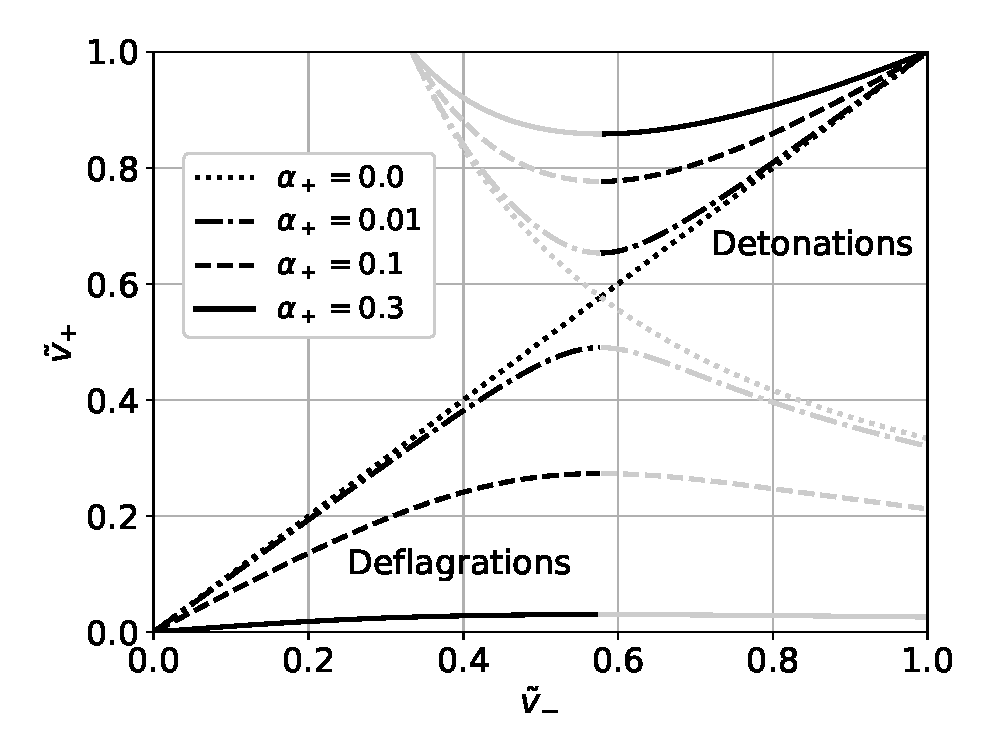
\includegraphics[width=0.7\textwidth]{../pttools/examples/fig/vm_vp_plane.eps}
\caption{Relation between the fluid velocity just ahead of the wall $\tilde{v}_+$ and just behind the wall $\tilde{v}_-$. Generated with PTtools. See also \cite[fig. 13]{lecture_notes}.}
\label{fig:vplus_vminus}
\end{figure}
\todo{Explain the blue points}

We can obtain useful continuity equations from the conservation of energy-momentum.
We start by defining two vectors, the fluid 4-velocity
\begin{equation}
u^\mu \equiv \gamma(-1, \overrightarrow{v})^\mu
\label{eq:u_mu}
\end{equation}
and its orthonormal vector
\begin{equation}
\bar{u}^\mu \equiv \gamma(-v, \frac{\overrightarrow{v}}{v})^\mu.
\end{equation}
\todo{Check the signs of the time components.}
Please note that the way these vectors are defined and the convention for the signature of the metric vary
from article to article.
These vectors form an orthonormal basis.
It should be noted, that for orthonormal vectors
% Note that the lecture notes use ubar here.
\begin{align}
u_\mu u^\mu &= -1, \\
u_\mu \bar{u}^\mu &= 0.
\end{align}
\cite[p. 36]{lecture_notes}
By projecting the conservation equation~\eqref{eq:ep_conservation} to this basis and noting that
$\nabla_\nu (u_\mu u^\mu) = 0$ and therefore $u_\mu \nabla_\nu u^\mu = 0$, we get
\cite[eq. 7.28-7.29]{lecture_notes}
\begin{align}
0 &= u_\mu \nabla_\nu T^{\mu \nu} = -\nabla_\mu (w u^\mu) + u^\mu \nabla_\mu p,
\label{eq:continuity1} \\
0 &= \bar{u}_\mu \nabla_\nu T^{\mu \nu} = w \bar{u}^\nu u^\mu \nabla_\mu u_\nu + \bar{u}^\mu \nabla_\mu p.
\label{eq:continuity2}
\end{align}
These are known as the continuity equations, or the hydrodynamic equations.
It should be noted that many articles use the symbol of a partial derivative $\partial$ in these equations,
even though it's actually a covariant derivative $\nabla$.
Since we are operating in spherical coordinates,
the divergence of a vector $A$ is given by
\begin{align}
\nabla \cdot A
% &= \partial_r A^r + \partial_\theta A^\theta + \partial_\phi A^\phi \\
&= \frac{1}{r^2} \frac{\partial (r^2 A^r)}{\partial r}
+ \frac{1}{r \sin \theta} \frac{\partial A^\theta}{\partial \theta}
+ \frac{1}{r \sin \theta} \frac{\partial A^\phi}{\partial \phi}.
\label{eq:divergence}
\end{align}
Let us look for a spherically symmetric self-similar solution using the dimensionless coordinate
\begin{equation}
\xi \equiv \frac{r}{t}.
\end{equation}
In a spherically symmetric case for $u^\mu$ of eq.~\eqref{eq:u_mu},
the latter two terms of~\eqref{eq:divergence} are zero, and therefore
\begin{equation}
\nabla_\mu u^\mu = \frac{\gamma}{t} \left[ 2\frac{v}{\xi} + \left[1 - \gamma^2 v (\xi - v) \right] \frac{\partial v}{\partial \xi} \right]
\end{equation}
The gradients in~\eqref{eq:continuity1} and~\eqref{eq:continuity2} can also be expressed as~\cite[eq. 25]{espinosa_energy_2010}.
\begin{align}
u_\mu \nabla^\mu &= - \frac{\gamma}{t} (\xi - v) \frac{\partial}{\partial \xi}, \\
\bar{u}_\mu \nabla^\mu &= \frac{\gamma}{t} (1 - \xi v) \frac{\partial}{\partial \xi}.
\end{align}
With these eq.~\eqref{eq:continuity1} and~\eqref{eq:continuity2} can be expressed as
\begin{align}
(\xi - v) \frac{1}{w} \frac{de}{d\xi} &= 2 \frac{v}{\xi} + \left[ 1 - \gamma^2 v (\xi - v) \right] \frac{dv}{d\xi}, \\
(1 - v\xi) \frac{d_\xi p}{w} &= \gamma^2 (\xi - v) \frac{dv}{d\xi}.
\end{align}
These are dependent only on $\xi$ instead of $r$,
and therefore a spherically symmetric self-similar solution exists.
Here the derivatives are now total derivatives, as $e$ and $p$ are functions of a single variable.
By dividing one equation by the other and using eq.~\eqref{eq:cs2_compact}, we can combine these to
\begin{equation}
2 \frac{v}{\xi} = \gamma^2 (1 - v\xi) \left[ \frac{\mu^2}{c_s^2} - 1 \right] \frac{dv}{d\xi},
\label{eq:continuity_combined}
\end{equation}
where
\begin{equation}
\mu(\xi,v) \equiv \frac{\xi - v}{1 - \xi v}
\label{eq:mu}
\end{equation}
is the
\href{https://en.wikipedia.org/wiki/Velocity-addition_formula#Standard_configuration}{Lorentz transformed fluid velocity}
$\xi$ in a frame moving outward with the speed $v$.
This can be rearranged to give
\cites[eq. 7.30-7.31]{lecture_notes}[eq. 5]{giese_2021}
\begin{equation}
\frac{dv}{d\xi} = \frac{2v(1-v^2)}{\xi(1-v\xi)} \left( \frac{\mu(\xi,v)^2}{c_s^2} - 1 \right)^{-1}.
\label{eq:hydro_diff1}
\end{equation}
From eq.~\eqref{eq:continuity2} using eq.~\eqref{eq:cs2_compact} and~\eqref{eq:enthalpy_sum} we also get
\begin{equation}
\frac{dw}{d\xi} = w \left( 1 + \frac{1}{c_s^2} \right) \gamma^2 \mu(\xi,v) \frac{dv}{d\xi}.
\label{eq:hydro_diff2}
\end{equation}

Equation~\eqref{eq:hydro_diff1} can be split in two using an auxiliary quantity $\tau$,
resulting in the equation group
\cite[eq. B.14-16]{hindmarsh_gw_pt_2019}
\begin{align}
\frac{d\xi}{d\tau} &= \xi \left[ (\xi - v)^2 - c_s^2 (1 - \xi v)^2 \right],
\label{eq:hydro_param1} \\
\frac{dv}{d\tau} &= 2 v c_s^2 (1 - v^2) (1 - \xi v),
\label{eq:hydro_param2} \\
\frac{dw}{d\tau} &= w \left( 1 + \frac{1}{c_s^2} \right) \gamma^2 \mu \frac{dv}{d\tau}.
\label{eq:hydro_param3}
\end{align}
This is easier to prove in the reverse direction by dividing one equation by the other.
It should be noted that in general $c_s^2 = c_s^2(w,\phi)$, which tightens the coupling between these equations.
The parametric equations have fixed points at
$(\xi,v) = (0,0)$ and
$(\xi,v) = (1,1)$.
When $c_s$ is a constant, the equations also have a fixed point at
$(\xi,v) = (c_s,0)$.
When $c_s$ is constant, the first two equations are not dependent on enthalpy, which simplifies the integration considerably.
However, in the general case of $c_s(w,\phi)$ the equations have to be integrated together.
\todo{Add $(\xi,v)$ plots to the models and refer to them here.}
